\documentclass[12pt]{report}
\usepackage[a4paper]{geometry}
\usepackage{fancyhdr}
\pagestyle{fancy}
\fancyhead[c]{}
\fancyhead[l]{\thechapter}
\fancyhead[r]{\thesection}

\fancyfoot[l]{}
\fancyfoot[c]{\thepage}
\fancyfoot[r]{}

\usepackage{microtype}
\usepackage{todonotes}

\usepackage{math-packages}
\usepackage{math-environments}
\usepackage{math-macros}
\usepackage{tikz}

% \usepackage{fontspec}
% \setmainfont{Gill Sans Light}

\usepackage[citestyle=alphabetic,
            bibstyle=authortitle,
            backend=biber]{biblatex}
\addbibresource{bibliography.bib}


\newenvironment{note}{\begin{bluebox}}{\end{bluebox}}
\newenvironment{warning}{\begin{redbox}}{\end{redbox}}
\makeindex


\title{Mathematics}
\author{James Leslie}
\date{\today}
\begin{document}
\listoftodos{}
\maketitle
\tableofcontents


\part{Algebra}
\chapter{Group Theory}\label{cha:intr-group-theory}
Group theory is the study of symmetries, or more abstractly, automorphisms.
%
Introduction to Group Theory was my first ``real'' taste of algebra at university.
%
It was half of the course Fundamental of Pure Mathematics, the other half being an introduction to real analysis.
%
I took this course in the second semester of my second year in 2015, and the group theory part was taught by \href{https://www.maths.gla.ac.uk/~mwemyss/}{Michael Wemyss}.
%
It was followed up by a fourth year course ``Group Theory''.


This chapter is based off the notes~\cite{wemyss2015grouptheory} and~\cite{lanini2017grouptheory}.


\section{Groups and Symmetries}
The study of any area of pure mathematics needs to be well motivated.
%
Group theory is really the study of automorphisms.
%
This becomes quite tangible when applied to concrete objects such as graphs, whose automorphisms are symmetries.


\begin{definition}\cite[Definition 1.1.1]{wemyss2015grouptheory}\label{def:intr-group-theory:graph}
  A \indx{graph} is a finite set of vertices, with at most one edge between any two vertices.
  %
  There are no self edges allowed.
\end{definition}

\begin{example}
  The following are examples of graphs.

  % TODO: Add more tikz graphs and tidy up.
  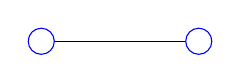
\begin{tikzpicture}
    \node[shape=circle, draw=blue] (A) at (-1,0) {};
    \node[shape=circle, draw=blue] (B) at (1,0) {};

    \path [-] (A) edge (B);
  \end{tikzpicture}
\end{example}

\begin{definition}\cite[Definition 1.1.3]{wemyss2015grouptheory}
  A symmetry of a graph is a bijection \(f : V \to V\) on such that \(f(v_{1})\) and \(f(v_{2})\) are joined by an edge if and only if \(v_{1}\) and \(v_{2}\) are joined by an edge.
\end{definition}

\begin{example}
  Determine all the symmetries of the following graph:

  \begin{centre}
    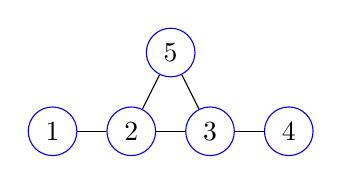
\begin{tikzpicture}
      \node[shape=circle, draw=blue] (1) at (0,0) {1};
      \node[shape=circle, draw=blue] (2) at (1,0) {2};
      \node[shape=circle, draw=blue] (3) at (2,0) {3};
      \node[shape=circle, draw=blue] (4) at (3,0) {4};
      \node[shape=circle, draw=blue] (5) at (1.5,1) {5};

      \path [-]  (1) edge (2);
      \path [-]  (2) edge (3);
      \path [-]  (3) edge (4);
      \path [-]  (2) edge (5);
      \path [-]  (3) edge (5);
    \end{tikzpicture}
  \end{centre}

  Let \(f\) be an arbitrary symmetry.
  %
  By definition, \(f\) must preserve the valency of vertices.
  %
  As vertex 5 is the only vertex of valency 2, we must have that \(f(5) = 5\).
  %
  Since vertices 2 and 3 are the only vertices of valency 3, \(f\) can either fix them, or swap them.
  \begin{enumerate}
  \item
    Suppose they are fixed.
    %
    Then \(f\) fixes both 1 and 4 as \(f(1)\) has valency 1 and must be connected to \(f(2) = 2\), hence \(f(1) = 1\).
    %
    A similar argument applies to vertex 4.
    %
    The completes the case where \(f\) fixes vertex 2 and 3.
  \item
    Suppose they are swapped.
    %
    Then \(f(1) = 4\), as \(f(1)\) must have valency 1 and be connected to \(f(3) = 3\).
    %
    Likewise, \(f(4) = 1\).
  \end{enumerate}

  Hence there are exactly two symmetries.
\end{example}

\begin{note}
  The definition of a symmetry is not dependent on the embedding of the graph in the plane.
  %
  It is easy to visually inspect a graph and gain an intuition about the symmetries, but a formal proof requires one to be more precise.
\end{note}


\section{Groups and examples}

\begin{definition}\label{def:intro-to-group-theory:group}
  A \indx{group} \(G\) is a set \(G\) equipped with a binary operation \(* : G \times G \to G\), a unary operation \((-)^{-1}: G \to G\), and an identity element \(e \in G\) such that the following properties hold:

  \begin{enumerate}
    \item \(*\) is associative (\((g * h) * j = g * (h * j)\));
    \item \(e * g = g = g * e\), for all \(g \in G\);
    \item \(g * g^{-1} = e = g^{-1} * g\).
  \end{enumerate}

  The \indx{order} of a group \(G\), denotes \(|G|\) is the cardinality of the underlying set.

  The \indx{order} of an element \(g \in G\) is the smallest natural number \(n\) such that \(g^{n} \coloneqq \underbrace{g * g * \ldots * g}_{n} = e\).
\end{definition}


\begin{example}
  The automorphisms of an object (i.e the symmetries of a graph) form a group.
\end{example}


\begin{example}
  The integers \(\Z\) form a group under addition.
\end{example}


\begin{example}\label{ex:group-theory:symmetric-group}
  \(S_{n}\), the \index{symmetric group} on \(n\) elements is the set of permutations of \(\{1, \ldots, n\}\).
  %
  It is a group under composition.


  We typically use cycle notation \((123)(12): S_{3} \to S_{3}\), where \((123)\) means the permutation sending 1 to 2, 2 to 3 and 3 to 1.
  %
  Two bracket cycles next to each other for a permutation by composition.
\end{example}

\begin{example}
  The \(n^{\text{th}}\) \indx{dihedral} group is the group of symmetries of the \(n\)-gon.
  %
  It has \(2n\) elements: \(n\) rotations and \(n\) reflections.

  \begin{centre}
    \begin{tikzpicture}
      \node[shape=circle, draw=blue] (A) at (-1,1) {};
      \node[shape=circle, draw=blue] (B) at (1,1) {};
      \node[shape=circle, draw=blue] (C) at (1,-1) {};
      \node[shape=circle, draw=blue] (D) at (-1,-1) {};

      \node[] (E) at (2,2) {};
      \node[] (F) at (-2,-2) {};
      \node[] (G) at (0,2) {};
      \node[] (H) at (0,-2) {};

      \path [-] (A) edge (B);
      \path [-] (B) edge (C);
      \path [-] (C) edge (D);
      \path [-] (D) edge (A);

      \path [-] (E) edge (F);
      \path [-] (G) edge (H);
    \end{tikzpicture}
  \end{centre}
\end{example}
\todo{add more examples}


\section{Subgroups and Lagrange's Theorem}

\begin{definition}\label{def:group-theory:subgroup}
  A \indx{subgroup} \(H\) of a group \(G\) is a subset \(H \subset G\) such that it is still a group under the restriction of the structure of \(G\) to \(H\).
  %
  That is, if the following hold:
  \begin{enumerate}
  \item For all \(h, k \in H\), \(hk \in H\);
  \item For all \(h \in H\), \(h^{-1} \in H\).
  \end{enumerate}


  We write \(H \leq G\) to say that \(H\) is a subgroup of \(G\).
\end{definition}


\begin{lemma}\label{lem:group-theory:subgroup-test}
  Let \(H \subset G\).
  %
  Then \(H \leq G\) if and only if \(hk^{-1} \in H\) for all \(h,k \in H\).
\end{lemma}


\begin{example}
  The group of rotations of an \(n\)-gon are a subgroup of \(D_{n}\).
\end{example}


\begin{example}
  The \(n\)-th \indx{alternating group}, denoted \(A_{n}\) is the subgroup of \(S_{n}\) consisting of all permutations that can be written as the product of an even number of 2-cycles.
\end{example}

\begin{example}
  Let \(F\) be a field.
  %
  The \indx{general linear group} \(GL(n, F)\) is the set of all invertible \(n \times n\) matrices over \(F\).
  %
  The \indx{special linear group} \(SL(n, F)\) is the set of all \(n \times n\) matrices over \(F\) with determinant \(1\).
  %
  It is a subgroup of \(GL(n, F)\).
\end{example}


An important construct from a subgroup \(H \leq G\) is that of the left and right cosets.

\begin{definition}\label{def:group-theory:coset}
  Let \(H \leq G\), and \(g \in G\).
  %
  The \indx{left coset} of \(H\) determined by \(g\) is the set \(gH \coloneqq \{gh \mid h \in H\}\).
  %
  Similarly, the \indx{right coset} of \(H\) determined by \(G\) is \(Hg\).


  The number of left cosets of a subgroup \(H \leq G\) is called the \indx{index} of \(H\) in \(G\), and is denoted \([G : H]\).
\end{definition}

\begin{example}
  Let \(G\) be a group and let \(g \in G\).
  %
  Then, \(\langle g \rangle \coloneqq \{g^{n} \mid n \in \Z\}\) is a subgroup of \(G\) called the \indx{subgroup generated by \(g\)}.
  %
  If \(G = \langle g \rangle\) for some \(g \in G\), then we say that \(G\) is \indx{cyclic}.
\end{example}

\begin{lemma}
  If \(G\) is a cyclic group, then either \(G \iso C_{n}\) for some \(n \in \N\) or \(G \iso (\Z, +)\).
\end{lemma}

The most important type of subgroup are the normal subgroups.

\begin{definition}
  A subgroup \(H \leq G\) is \indx{normal} if \(gH = Hg\) for all \(g \in G\).
  %
  We write \(H \triangleleft G\) to say that \(H\) is normal in \(G\).
\end{definition}

We reach the titular theorem of this section.

\begin{theorem}[Lagrange's Theorem]
  Let \(H\) be a subgroup of a finite group \(G\). Then
  \[|G| = [G : H]|H|.\]
\end{theorem}

\begin{proof}
  This follows from the fact that the cosets of a subgroup \(H\) partition \(G\), and each coset has the same size.


  Suppose that \(g \in aH\) and \(g \in bH\), for some \(a, b \in G\).
  %
  Then some simple algebra shows that \(a \in bH\) and \(b \in aH\), from which we deduce that \(a = b h_{1}\) and \(b = a h_{2}\) for some \(h_{1}, h_{2} \in H\).
  %
  Then any \(ah \in aH\) is equal to \(bh_{1}h \in bH\), so \(aH \subset bH\).
  %
  Similarly, we can show that \(bH \subset aH\), and so \(aH = bH\).
  %
  Therefore \(aH = bH\) or \(aH \cap bH = \emptyset\).
  %
  It is also clear that every \(g \in G\) is in \(gH\), and so cosets partition \(G\).


  It is also clear that the function \(ah_{1} \mapsto bh_{1}\)  from \(aH \to bH\) is a bijection, and so any two left cosets of H have the same cardinality.

  This completes the proof of Lagrange's Theorem.
\end{proof}



\begin{corollary}
\label{cor:group-theory:order-divides-group}
  Suppose \(G\) is a finite group and \(g \in G\).
  %
  Then, \(o(g) \mid \left|G\right|\).
\end{corollary}

\begin{proof}
  The subgroup \(\langle g \rangle \leq G\) has order \(o(g)\), and so by Lagrange's theorem, \(o(g)\) must divide \(|G|\).
\end{proof}

\begin{corollary}
\label{cor:group-theory:g-to-power-of-group-order-is-e}
  Suppose \(G\) is a finite group.
  %
  For all \(g \in G\), \(g^{\abs{G}} = e\).
\end{corollary}

\begin{proof}
  By Corollary~\ref{cor:group-theory:order-divides-group}, \(|G| = k \times o(g)\), for a fixed \(g \in G\).
  %
  Then, \(g^{\abs{G}} = g^{k \times o(g)} = e^{k} = e\).
\end{proof}

\begin{corollary}
  Let \(G\) be a finite group.
  %
  If \(\abs{G}\) is prime, then \(G\) is cyclic.
\end{corollary}

\begin{proof}
  If \(\abs{G}\) is prime, the only subgroups are \(\{e\}\) and \(G\).
  %
  Since \(\langle g \rangle \leq G\) is non-trivial for non-identity elements \(g \in G\), it must be the whole group.
  %
  Therefore, \(G\) is equal to a cyclic subgroup and is cyclic itself.
\end{proof}


Lagrange's Theorem can be used to prove Fermat's second most famous theorem.

\begin{theorem}
 \label{thm:group-theory:fermats-little-theorem}
 If \(p\) is a prime and \(a \in \Z\), then
 \[a^{p} \equiv a \mod p.\]
\end{theorem}

\begin{proof}
  This holds trivially for \(a = 0\), so assume \(a \not\equiv 0 mod p\).
  %
  Then, \(g\) is in the multiplicative group of units \(\Z^{*}_{p}\), which has order \(p-1\). By Corollary~\ref{cor:group-theory:g-to-power-of-group-order-is-e}, \(a^{p-1} \equiv 1 \mod p\), and so \(a^{p} \equiv a \mod p\).
\end{proof}

Wilson's Theorem also follows as an application of Lagrange's Theorem.

\begin{theorem}[Wilson's Theorem]
  \label{thm:group-theory:wilsons-theorem}
  If \(p\) is a prime number then the following hold:
  \begin{enumerate}
  \item
    In \(\Z^{*}_{p}\), only \(1\) and \(p-1\) are their own inverses.
  \item
    \((p - 1)! \equiv -1 \mod p\).
  \end{enumerate}
\end{theorem}

\begin{proof}
  We prove both parts.
  \begin{enumerate}
  \item
    Clearly, 1 and \(p-1\) are their own inverses.
    %
    Take \(1 < a < p -1\).
    %
    Neither \(a-1\) nor \(a+1\) are multiples of \(p\) and as \(p\) is prime, \((a-1)(a+1) = a^{2} -1\) is not a multiple of \(p\).
    %
    Therefore, \(a^{2}-1 \not\equiv 0 \mod p\), and so \(a^{2} \not\equiv 1 \mod p\) proving that \(a\) is not its own inverse.

  \item
    This follows by a simple counting argument.
    %
    Every element \(a \in \{2, \ldots, p-2\}\) can be paired up with its inverse, which is also in that range.
    %
    Therefore, the product \((p-1)! \equiv p-1 \equiv -1 \mod p\).
  \end{enumerate}
\end{proof}


\section{Group homomorphisms}
\label{sec:group-theory:group-homomorphisms}

We now turn to the morphisms between groups.

\begin{definition}
  \label{def:group-theory:group-homomorphism}
  Let \(G, H\) be groups.
  %
  A function \(\phi : G \to H\) such that \(\phi(ab) = \phi(a) \phi(b)\), for all \(a, b \in G\) is a \indx{group homomorphism}.
\end{definition}

\begin{lemma}
  Let \(\phi : G \to H\) be a group homomorphism.
  %
  Then the following hold:
  \begin{enumerate}
  \item
    \(\phi(e) = e\) and \(\phi(g^{-1}) = \phi(g) ^{-1}\).
  \item
    If \(\phi\) is injective, then \(o(g) = o\left(\phi(g)\right)\).
  \end{enumerate}
\end{lemma}

\begin{proof}
  \begin{enumerate}
  \item
    We have the following equalities hold:
    \begin{align*}
      \phi(e) &= \phi(ee) \\
              &= \phi(e) \phi(e).
    \end{align*}
    %
    Therefore, we can apply \(\phi(e)^{-1}\) to both sides of the equation and cancel to get \(\phi(e) = e\).
    %
    Recalling that inverses are unique, \(\phi(g)\phi(g^{-1}) = \phi(gg^{-1}) = \phi(e) = e\).
    %
    Applying the similar proof by multiplying \(\phi(g)\) on the left, we deduce that \(\phi(g^{-1}) - \phi(g)^{-1}\).

  \item
    Suppose that \(o(\phi(g)) = n\).
    %
    Then, \(e = \phi(e) = \phi(g)^{n} = \phi(g^{n})\), and so by injectivity of \(\phi\), \(e = g^{n}\).
    %
    Suppose there exists \(0 < k < n\) such that \(g^{k} = e\). Then, \(e = \phi(e) = \phi(g^{k}) = \phi(g)^{k}\), which contradicts \(n\) being the order of \(o(\phi(g))\). Hence \(n\) is the order of \(g\).

  \end{enumerate}
\end{proof}

\begin{example}
  Let \(C_{n}\) be the \indx{cyclic group of order \(n\)}, which is defined as the set of rotations of the equilateral \(n\)-gon.
  %
  If \(g\) is a rotation by \(2 \pi /n \) radians, then \(C_{n} \coloneqq \langle g \rangle\).
  %
  The function
  \begin{align*}
    \phi : \Z &\to C_{n} \\
    a &\mapsto g^{a}
  \end{align*}
  is a group homomorphism.
\end{example}


\begin{definition}
  \label{def:group-theory:group-isomorphism}
  Let \(G, H\) be groups and \(\psi : G \to H\) a group homomorphism.
  %
  We say that \(\phi\) is a \indx{group isomorphism} if there is a group homomorphism \(\psi\) such that \(phi\) and \(\psi\) are inverse functions.

  If there exists an isomorphism \(\psi : G \to H\), we say \(G\) and \(H\) are \indx{isomorphic as groups}, and write \(G \iso H\).
\end{definition}

\begin{lemma}
  \label{lem:group-theory:groups-of-order-p-are-isomorphic}
  If \(p\) is a prime number, then all groups of order \(p\) are isomorphic.
\end{lemma}

\begin{proof}
  Let \(G, H\) be groups of order \(p\).
  %
  Then, every non-identity element has order \(p\), since by Lagrange's Theorem every non-trivial subgroup is equal to the whole group.
  %
  Choose a non-identity element \(g \in G\) and \(h \in H\).
  %
  The function mapping \(g^{n} \mapsto h^{n}\) is well defined and is a bijective group homomorphism.
  %
  Hence, \(G \iso H\).
\end{proof}

\begin{lemma}
  All cyclic groups of order \(n\) are isomorphic.
\end{lemma}

\begin{proof}
  This is the same proof as Lemma~\ref{lem:group-theory:groups-of-order-p-are-isomorphic}.
\end{proof}


Given a group homomorphism, we can always extract a new group from it.

\begin{definition}
  Let \(\phi:G \to H\) be a group homomorphism.
  %
  The \indx{kernel} of \(\phi\) is the subset \(\{g \in G \mid \phi(g_) = e\}\).
\end{definition}

\begin{lemma}
  The kernel of a homomorphism \(\phi : G \to H\) (denoted \(\ker(\phi)\)) is a subgroup of \(G\).
\end{lemma}

\begin{proof}
 Clearly, for all \(g, h \in \ker(\phi)\) we have that \(\phi(gh^{-1}) = \phi(g)\phi(h)^{-1} = e\), and as \(e \in \ket(\phi)\), \(\ker(\phi)\) is a subgroup of \(G\).
\end{proof}




















\chapter{Introduction to Number Theory}\label{cha:intr-numb-theory}
\chapter{Honours Algebra}\label{cha:honours-algebra}
\chapter{Commutative Algebra}\label{cha:commutative-algebra}
\chapter{Galois Theory}\label{cha:galois-theory}
\chapter{Lie Algebras}\label{cha:lie-algebras}



\part{Analysis and calculus}
\chapter{Calculus}\label{cha:calculus}
\chapter{Introduction to Real Analysis}\label{cha:intr-real-analys}
\chapter{Honours Analysis}\label{cha:honours-analysis}
\chapter{Complex Variables}\label{cha:complex-variables}
\chapter{Honours Differential Equations}\label{cha:hono-diff-equat}
\chapter{Essentials in Analysis and Probability\label{cha:essent-analys-prob}}
\chapter{Linear Analysis}\label{cha:linear-analysis}
\chapter{Fourier Analysis}\label{cha:fourier-analysis}
\chapter{Quantum Information}\label{cha:quantum-information}
\chapter{Variational Calculus}\label{cha:variational-calculus}

\part{Combinatorics, probability and statistics}
\chapter{Probability with Applications}\label{cha:prob-with-appl}
\chapter{Statistics}\label{cha:statistics}
\chapter{Combinatorics and Graph Theory}\label{cha:comb-graph-theory}

\part{Topology and Geometry}
\chapter{Geometry}\label{cha:geometry}
\chapter{General Topology}\label{cha:general-topology}
\chapter{Algebraic Topology}\label{cha:algebraic-topology}
\chapter{Algebraic Geometry}\label{cha:algebraic-geometry}
\chapter{Complex Algebraic Curves}\label{cha:compl-algebr-curv}




\part{Category Theory and its Applications}\label{part:category-theory-its}
\chapter{Category Theory}\label{cha:category-theory}
\chapter{Homotopy Theory}\label{cha:homotopy-theory}
\chapter{Higher Category Theory}\label{cha:high-categ-theory}
\chapter{Multidimensional Category Theory}\label{cha:mult-categ-theory}

\printindex
\printbibliography%
\end{document}
